\documentclass{beamer}
\usetheme{Madrid}
\usecolortheme{beaver}

% Set graphics location
\graphicspath{ {Images/} }

%Information to be included in the title page:
\title{Structural Quality \& Software Evolution}
\author{Alison Major}
\institute{Lewis University}
\date{2022}

% \logo{
%   
\includegraphics[width=0.2\textwidth]{UniversityLogo}
% }

\begin{document}

\frame{\titlepage}

% 1 Introduction
% 1.1 Maintainability Index and Pylint Refactor Scores
% 1.2 Paper Structure
\begin{frame}
  \frametitle{Introduction}
  \textbf{Maintainability Index and Refactor Scores}
  \begin{itemize}
    \vspace{0.35cm}
    \item Areas of concern: cost, timeline, quality
    
    \vspace{0.35cm}
    \item Quality is hard to understand
    
    \vspace{0.35cm}
    \item Pylint \& Radon are a static analysis tools
    
    \vspace{0.35cm}
    \item Refactor violations point out code smells
  \end{itemize}
\end{frame}

% 2 Background and Literature Review

% 2.1 Keeping Users Engaged Long Term
% 2.1.1 Why does software evolution matter?
% 2.1.2 How do we ensure software evolution?
\begin{frame}
  \frametitle{Keeping Users Engaged Long Term}
  \textbf{Why does software evolution matter?}
  \begin{itemize}
    \item Users find bugs
    \item Users want new features
    \item New security threats
    \item New laws from governing bodies
  \end{itemize}
  
  \vspace{0.5cm}
  Need a thriving community of engaged users in order to keep apps and games successful.

  \vspace{0.35cm}
  In an open source system, need a thriving community of engaged developers in order to continue evolving.
\end{frame}

\begin{frame}
  \frametitle{Keeping Users Engaged Long Term}
  \textbf{How do we ensure software evolution?}

  \vspace{0.35cm}
  Keep the project maintainable.
  \begin{itemize}
    \item Bugs should be quick and easy to fix
    \item New features should be easy to add
    \item Consistent standards (naming, small methods, etc)
  \end{itemize}

  \vspace{0.5cm}
  \textbf{Software Maintenance}
  \newline Large portion of project cost in a typical software system is in the maintenance phase.
\end{frame}

\begin{frame}
  \frametitle{The Impact of Structural Quality}
  \textbf{Measuring Maintainability}
  \begin{itemize}
    \vspace{0.35cm}
    \item Easy to maintain = Easy to evolve
    
    \vspace{0.35cm}
    \item Pylint \& Radon Maintainability Index (MI)
    
    \vspace{0.35cm}
    \item Refactor Messages (Pylint)
    \begin{itemize}
      \item Refactor warnings are generally ``code smells''
      \item Code smells point out problems in Architecture
    \end{itemize}

    \vspace{0.35cm}
    \item PEP 8 is a set of Python standards
  \end{itemize}
\end{frame}

\begin{frame}
  \frametitle{The Impact of Structural Quality}
  \textbf{Other Maintainability Characteristics}
  \begin{itemize}
    \vspace{0.35cm}
    \item Low coupling, high cohesion
    
    \vspace{0.35cm}
    \item Confidence that metrics around software structure provide value in keeping systems maintainable (and therefore can evolve) % \cite{zhou:2020}
    
    \vspace{0.35cm}
    \item Readability
    \begin{itemize}
      \item Big commits reduce maintainability
      \item PEP 8 enforces readability
    \end{itemize}
  \end{itemize}
\end{frame}

\begin{frame}
  \frametitle{The Impact of Structural Quality}
  \textbf{Documentation and Maintainability}
  \begin{itemize}
    \vspace{0.35cm}
    \item Documentation holds the results of significant design decisions
    
    \vspace{0.35cm}
    \item Can influence the ability to evolve because\dots
    \begin{itemize}
      \item Enhances code understanding
      \item Comprehensibility impacts maintainability in a positive way  
    \end{itemize}
  \end{itemize}
\end{frame}

\begin{frame}
  \frametitle{Related Work}
  \textbf{Design Patterns and Software Quality}
  \begin{itemize}
    \vspace{0.35cm}
    \item Design patterns provide flexibility
    
    \vspace{0.35cm}
    \item Classes with frequent changes
    \begin{itemize}
      \item Easy to extend (okay)
      \item Correlates to other classes (high coupling... red flag!)
    \end{itemize}
    
    \vspace{0.35cm}
    \item We look at refactor score (code smell) not error score (bugs)
  \end{itemize}
  
  \vspace{0.35cm}
  Keeping this in mind, we focus on \emph{changes for system extensions and adaptiation}, not bug fixes.
\end{frame}

\begin{frame}
  \frametitle{Related Work}
  \textbf{Software Architecture and Maintainability}
  \begin{itemize}
    \vspace{0.35cm}
    \item Maintainability
    
    \vspace{0.35cm}
    \item Extensibility
    
    \vspace{0.35cm}
    \item Simplicity, understanding
    
    \vspace{0.35cm}
    \item Re-usability
    
    \vspace{0.35cm}
    \item Performance
  \end{itemize}

  \vspace{0.35cm}
  {\small \emph{Keep these in mind for easier future development when adding or changing code.}}
\end{frame}

% 3 Methodology
% 3.1 Initial Repository Set
% 3.2 Filtered Respository Set
\begin{frame}
  \frametitle{Methodology}
  \textbf{Initial Repository Set}
  \begin{itemize}
    \item Popular
    \item Long development history
    \item Multiple release cycles
  \end{itemize}

  \vspace{0.35cm}
  \textbf{Filtered Respository Set}
  
  \emph{At least 80\% Python code and top 20th percentile in these categories:}
  \begin{itemize}
    \item Long history of commits (2,968+ commits)
    \item Large number of contributors (90+ contributors)
    \item Many releases (44+ releases)
    \item Substantial Age (66.4+ months)
  \end{itemize}

  \vspace{0.35cm}
  Results in 46 repositories for further research.
\end{frame}

% 4 Results
\begin{frame}
  \frametitle{Results}
  \begin{itemize}
    \item Radon MI for all repositories rank as grade ``A''
    \newline which is considered ``very high maintainability''
    \item Open source systems with engaged community 
    \newline of developers tend to have higher scores
    \item For comparison, calculated ratio of refactor message count 
    \newline to SLOC as well as the average MI for a project.
  \end{itemize}

  \vspace{0.25cm}
  \begin{center}
    \begin{tabular}{ c c c c }
      \textbf{Repo} & \textbf{Ratio} & \textbf{Avg MI} & \textbf{Status} \\ 
      \hline\hline
      cython & 0.14 & 31.0 & active \\ \hline  % Best
      youtube-dl & 0.15 & 54.16 & active \\ \hline  % 2nd Best
      electrum & 0.16 & 39.41 & active \\ \hline  % 3rd Best
      \hline
      numba & 0.62 & 62.55 & active \\ \hline  % 3rd Worst
      scrapy & 0.64 & 64.47 & active \\ \hline  % 2nd Worst
      raven-python & 1.35 & 87.02 & deprecated \\ \hline  % Worst
    \end{tabular}
  \end{center}
\end{frame}

\begin{frame}
  \frametitle{Results}
  \begin{center}
    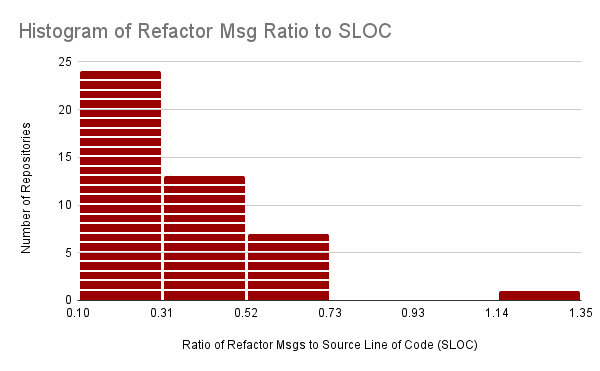
\includegraphics[width=0.8\columnwidth]{Histogram of Refactor Msg Ratio to SLOC.png}
  \end{center}
  \begin{center}
    {\small \emph{Diligent development communities can keep refactor warnings low,}}
    
    {\small \emph{regardless of system size (lines of code).}}
  \end{center}
\end{frame}

\begin{frame}
  \frametitle{Results}
  \begin{center}
    % 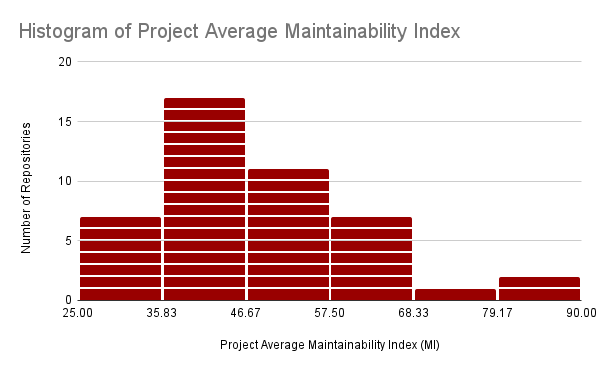
\includegraphics[width=0.8\columnwidth]{Histogram of Project Average Maintainability Index.png}
    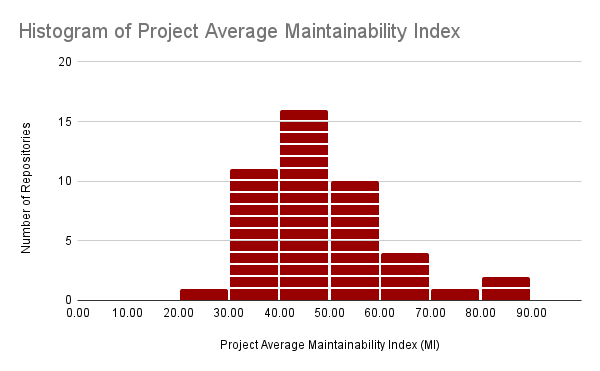
\includegraphics[width=0.8\columnwidth]{Histogram of Project Average Maintainability Index_BucketSize_10.png}
  \end{center}
  \begin{center}
    {\small \emph{Many repositories average in the mid-score to high-score.}} 
    
    {\small \emph{Radon considers 20 points and up to be very maintainable.}}
  \end{center}
\end{frame}

% 5 Conclusions and Recommendations
\begin{frame}
  \frametitle{Conclusions}
  \begin{itemize}
    \item Structural quality impacts software evolution.
    
    \vspace{0.35cm}
    \item Good projects will grow and evolve.
    
    \vspace{0.35cm}
    \item Poor structure leads to deprecation.
    \begin{itemize}
      \item If the development community is engaged, deprecation of 
        \newline the project may lead to a fresh, improved code base.
    \end{itemize}
    
    \vspace{0.35cm}
    \item Open source and projects with many contributors are vulnerable to degrading maintainability.
    \begin{itemize}
      \item Popular repositories with a long history of commits and releases 
        \newline (i.e. our repository data set) tend to have good maintainability.
      \item The high maintainability is a testament to their longevity.
    \end{itemize}
  \end{itemize}
\end{frame}

\begin{frame}
  \frametitle{Recommendations}
  \begin{itemize}
    \item Good architecture is important for evolution.
    
    \vspace{0.35cm}    
    \item Reliable quality metric can be a useful way to measure maintainability, which promotes ability to evolve a project.
    
    \vspace{0.35cm}
    \item Pick a set of standards to maintain good architecture even with a large, open source community.
    \begin{itemize}
      \item Limit complexity as project changes and grows.
      \item SOLID principles.
      \item Keep it DRY.
      \item And other design patterns known to be best practice.
    \end{itemize}
    
    \vspace{0.35cm}
    \item Auto-enforce by using quality measurements for desired standards in the project's CI/CD pipeline.
  \end{itemize}
\end{frame}

\end{document}